\documentclass{article}

% Language setting
% Replace `english' with e.g. `spanish' to change the document language
\usepackage[french]{babel}
\usepackage[fleqn]{amsmath} % Aligner les équations à gauche


% Set page size and margins
% Replace `letterpaper' with`a4paper' for UK/EU standard size
\usepackage[letterpaper,top=2cm,bottom=2cm,left=3cm,right=3cm,marginparwidth=1.75cm]{geometry}

% Useful packages

\usepackage{amsmath}
\usepackage{amssymb}
\usepackage{graphicx}
\usepackage{subcaption}
\usepackage[colorlinks=true, allcolors=blue]{hyperref}

\title{TD 5 - Electrostatique}
\author{IPESUP - PC }
\date{09/10/2024}

\begin{document}
\maketitle

\section{Rappels de cours}

Soit deux charges ($q_1 \text{ et } q_2$) séparées par une distance $r$, la force électrostatique entre ces deux charges est donnée par la loi de Coulomb:\\[0.2cm]
$F_{1 \rightarrow 2} = \frac{1}{4\pi \varepsilon_0} \frac{q_1 q_2}{r^2} \vec{u}_{1 \rightarrow 2}$\\
$\epsilon_0 = 8.85 \times 10^{-12} { F.m^{-1}}$\\[0.1cm]

\textbf{Champ électrique:}\\[0.1cm]
Soit une charge $q$ en $0$ et un point $M$ de l'espace, le champ électrique en $M$ est donné par:\\
$\vec{E}(M) = \frac{1}{4\pi \varepsilon_0} \frac{q}{r^2} \vec{u}_{0 \rightarrow M}$\\

\textbf{Potentiel électrique:} On dit que $\vec{E}(M)$ dérive du potentiel $V(M)$ si $\vec{E} \cdot \vec{OM} = -dV$.\\[0.1cm]

\textbf{Ligne de champ: } C'est une courbe tangente en chaque point au vecteur champ électrique.\\[0.1cm]
Propriétés: 
\begin{enumerate}
    \item Les lignes de champ sont orientées selon les potentiels décroissants.
    \item Les lignes de champ sont orthogonales aux surfaces équipotentielles.\\
\end{enumerate}

\textbf{Symétrie de champ: }\\[0.1cm]
Soit $S$ une rotation ou une symétrie (une isométrie de $\mathbb{R}^3$). Si la distribution  de charge est invariante par $S$, alors, $\forall M, \vec{E}(S(M)) = S(\vec{E}(M))$\\ 

\textbf{Théorème de Gauss: }\\[0.1cm]
Soit une surface \textbf{fermée} $S$ de normale \textbf{extérieure} contenant une charge totale $q_int$. Soit $\vec{E}$ le champ électrique, le flux de $\vec{E}$ à travers $S$ est donné par:\\
$\Phi = \iint_S \vec{E} \cdot d\vec{S} = \frac{q_{int}}{\varepsilon_0}$\\


\textbf{Forme locale du théorème de Gauss:}\\[0.1cm]

$div(\vec{E}(M)) = \frac{\rho(M)}{\varepsilon_0}$\\

On utilisera la forme local dans le cas de discountinuité de la répartition de charge(charge linéique ou surfacique). Sinon, on utilisera la forme intégrale.\\

\textbf{Equation de Poisson:}\\[0.1cm]

Soit un champ électrique $\vec{E}$, le potentiel électrique $V$ est solution de l'équation de Poisson:\\
$\Delta V (M) = -\frac{\rho(M)}{\varepsilon_0}$\\

\textbf{Anecdote:}\\[0.1cm]
Pourquoi les passagers d'un avion ne sont pas électrisés lorsqu'un éclair frappe l'avion ? 
On peut comprendre cela grâce au théorème de Gauss. 
En effet, lorsque la foudre frappe l'avion, sa surface (conductrice) se charge fortement, il forme une \textbf{cage de Faraday}.
Cependant, l'intérieur est en isolant. On pourrait penser que les fortes charges créeraient un champ électrique dangereux, mais le théorème de Gauss nous dit que le champ à l'intérieur de l'avion est nul. 
Les passagers ne sont donc pas électrisés !\\[0.1cm]

\section{Calculs de champs:  }

\begin{enumerate}
    \item On considère une boule chargée de rayon $a$ et de densité volumique de charge $\rho(r, \theta, \phi) = \rho_0 \frac{r}{a}$ pour $0<r<a$. Déterminer le champ dans tout l'espace au moyens du théorème de Gauss et de sa forme locale.\\
    \item On considère un semi-conducteur orienté selon l'axe $Ox$, de surface $S$. Sa charge est nulle, sauf entre les plans $x=-a$ et $x=a$, où la densité de charge vaut $\rho(x, y, z) = \rho_0 sin(\frac{\pi x}{a})$. Déterminer le champ électrique dans tout l'espace. On considérera $a<<\sqrt{S}$. 
\end{enumerate}

On donne la divergence en coordonnées sphériques :\\[0.1cm] 

div($\vec{f}$) $=\frac{1}{r^2} \frac{\partial}{\partial r}(r^2 f_r) + \frac{1}{r \sin \theta} \frac{\partial}{\partial \theta}(\sin \theta f_\theta) + \frac{1}{r \sin \theta} \frac{\partial f_\phi}{\partial \phi}$

\section{Potentiel de Yukawa} 
Soit $\rho(r)$ une distribution de charge à symétrie sphérique créant le potentiel $V(r) = \frac{q^*e^{-\frac{r}{a}}}{4 \pi \varepsilon_0 r }$.
\begin{enumerate}
    \item Déterminer le champ électrique dans tout l'espace et en donner un équivalent pour $r \rightarrow 0$. Que pense-t-on de la distribution de charge en 0 ? 
    \item En utilisant le théorème de Gauss, montrer que $\rho(r) = \varepsilon_0 \frac{1}{r^2} \frac{d}{dr}(r^2 E(r))$. En déduire $\rho(r)$. 
    \item Calculer la charge totale contenue dans une sphère de rayon $R$ centrée en 0.
    \item En déduire la charge au centre.
\end{enumerate}


\section{Mer de Lidenbrock:}

On considère la Terre (supposée ronde), de rayon $R$ et de centre $O$. A l'intérieur se trouve une cavité sphérique de centre $O' \neq O $ et de rayon $a < \left\lVert \vec{OO'}\right\rVert $. 
Par analogie avec la force électrostatique, déterminer un théorème de Gauss pour la force gravitationelle puis en déduire le champ gravitationnel créé par une boule homogène dans tout l'espace. 
En déduire le champ de gravitation à l'intérieur de la cavité. \\





\begin{figure}[h]
  \centering
  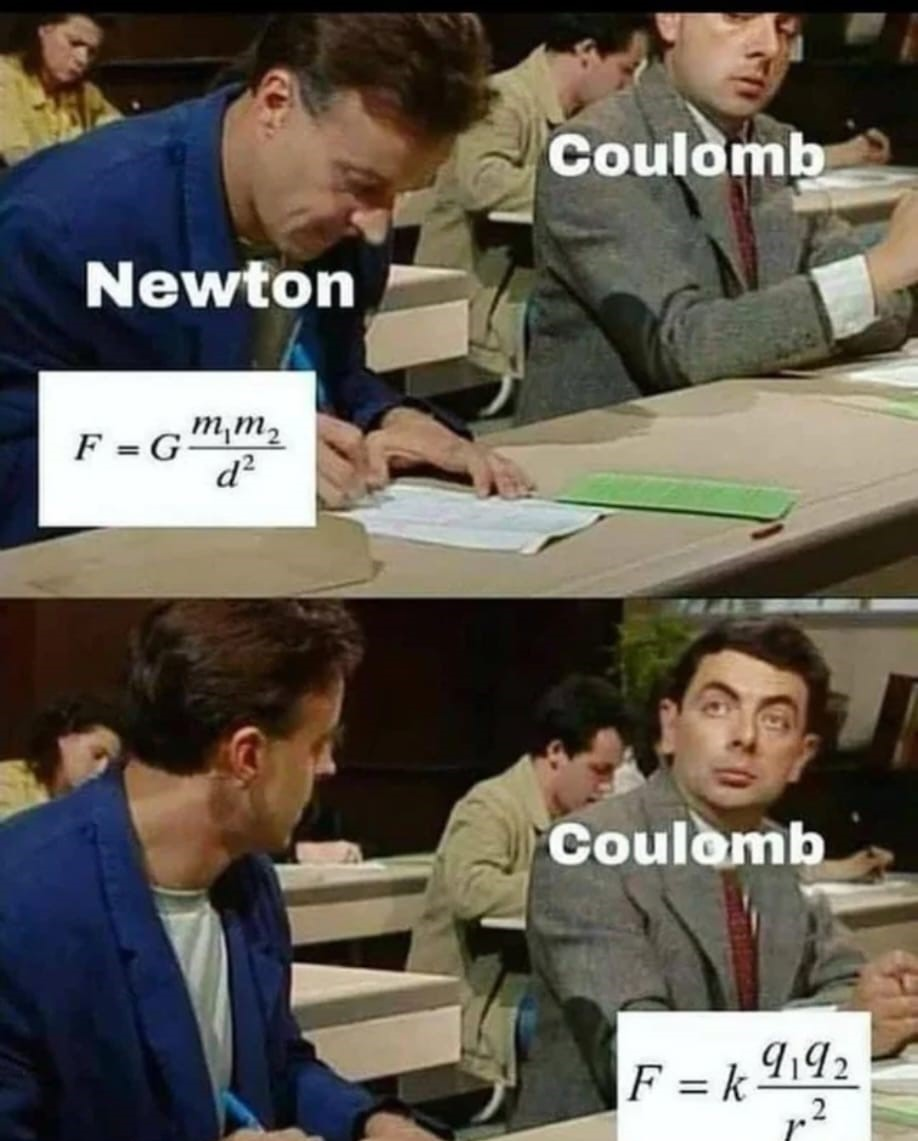
\includegraphics[width=0.3\textwidth]{meme.jpg}
  \label{fig:maison}
\end{figure}



\end{document}

